\documentclass[11pt,a4paper]{article}

% Packages
\usepackage[utf8]{inputenc}
\usepackage[T1]{fontenc}
\usepackage{lmodern}
\usepackage{amsmath,amssymb,amsthm}
\usepackage{enumitem}
\usepackage{geometry}
\usepackage{titlesec}
\usepackage{xcolor}
\usepackage{fancyhdr}
\usepackage{graphicx}
\usepackage{booktabs}
\usepackage{float}
\usepackage[hidelinks]{hyperref}

% Page geometry
\geometry{
    a4paper,
    margin=0.9in
}

% Colors
\definecolor{customblue}{RGB}{0,102,204}

% Compact lists
\setlist[itemize]{
    leftmargin=*,
    topsep=2pt,
    itemsep=1pt,
    parsep=0pt
}
\setlist[enumerate]{
    leftmargin=*,
    topsep=2pt,
    itemsep=1pt,
    parsep=0pt
}

% Section formatting
\titleformat{\section}
    {\large\bfseries\color{customblue}}
    {}
    {0em}
    {}

\titleformat{\subsection}
    {\normalsize\bfseries\color{customblue}}
    {}
    {0em}
    {}

% Reduce spacing around headings
\titlespacing*{\section}{0pt}{8pt}{4pt}
\titlespacing*{\subsection}{0pt}{5pt}{2pt}

\setlength{\headheight}{14pt}

% Paragraph spacing
\setlength{\parindent}{0pt}
\setlength{\parskip}{3pt}

% Theorem environments
\newtheorem{theorem}{Theorem}
\newtheorem{lemma}[theorem]{Lemma}

% Notation
\newcommand{\Zp}{\mathbb{Z}_p}
\newcommand{\Zpx}{\mathbb{Z}_p[x]}

% Header
\pagestyle{fancy}
\fancyhf{}
\renewcommand{\headrulewidth}{0.4pt}
\fancyhead[L]{\textit{KerSplit}}
\fancyhead[R]{\thepage}

\title{\vspace{-2.4cm}\textbf{KerSplit}\\[6pt]
       \large Factoring Polynomials over $\mathbb{Z}_p$ with Berlekamp's Algorithm \\[4pt]
       \normalsize CS5610 Computational Number Theory and Algebra, IIT Hyderabad, 2026 \\[9pt]
       \begin{tabular}{ccc}Sai Deepak & Arjun Konidala & Ram Panikar \\ \small cs23btech11055 & \small cs23btech11026 & \small cs23btech11040\end{tabular}}
\author{}
\date{}

\begin{document}

\maketitle
\vspace{-1.0cm}

% -------------------------------------------------------
\section*{1. Background}
% -------------------------------------------------------

Factoring a polynomial over a finite field is one of the basic problems of computational
algebra. It is the inner step of factoring polynomials over $\mathbb{Z}$ and over number fields
(factor modulo a prime, then lift), and it appears in decoding BCH and Reed-Solomon codes, in
building extension fields $\mathbb{F}_{p^k}$, and in computing discrete logarithms. Unlike
factoring integers, it can be done in randomized polynomial time.

In the course (notes, Ch.~7) we solved the problem with the Cantor-Zassenhaus algorithm: reduce
to a square-free polynomial, separate the factors by degree (distinct-degree factorization), and
then split factors of equal degree with random gcds. We implemented it in Programming HW3.

Berlekamp's algorithm (1967) \cite{berlekamp67} was the first practical algorithm for this
problem and takes a different route. After the square-free step, it turns factoring into
\textbf{linear algebra over $\Zp$}. It builds a $d \times d$ matrix $Q$ from $f$. The null space of
$Q - I$ tells us \emph{how many} irreducible factors $f$ has before any factor is found, and its
elements split $f$ by gcds. The project name \emph{KerSplit} is the algorithm in two words:
compute a \textbf{kernel}, then \textbf{split}.

% -------------------------------------------------------
\section*{2. Problem Statement}
% -------------------------------------------------------

\subsection*{2.1 Statement}

\textbf{Input:} a prime $p$ and a non-zero polynomial $f \in \Zpx$ of degree $d$, in the
\texttt{p:}\,/\,\texttt{d:}\,/\,\texttt{f:} format of Programming HW3.

\textbf{Output:} the complete factorization
\[
  f = c \cdot h_1^{e_1} h_2^{e_2} \cdots h_k^{e_k},
\]
where $c \in \Zp^{*}$ is the leading coefficient, the $h_i$ are distinct monic irreducible
polynomials and $e_i \ge 1$, computed with Berlekamp's algorithm. For each square-free part the
program also reports $r$, the number of irreducible factors, which Berlekamp's method finds first.

Beyond correctness we ask one question: \emph{how does the cost of Berlekamp's algorithm depend on
$d$ and $p$, and how does it compare with Cantor-Zassenhaus on the same inputs?}

\subsection*{2.2 Scope}

\textbf{In scope}
\begin{itemize}
    \item Square-free decomposition with multiplicities, including factors $h^p$ whose derivative vanishes.
    \item The Berlekamp matrix $Q$ and the null space of $Q - I$ by our own Gaussian elimination over $\Zp$.
    \item The deterministic split (small $p$) and the randomized split (large $p$, including 512-bit primes), with $p = 2$ handled.
    \item A command-line program for HW3-format input with a step-by-step trace, a test suite, benchmarks against our HW3 Cantor-Zassenhaus, and a presentation notebook.
\end{itemize}

\textbf{Out of scope}
\begin{itemize}
    \item Factoring over $\mathbb{Z}$ (Hensel lifting, LLL) and over extension fields $\mathbb{F}_{p^k}$.
    \item Asymptotically fast variants (Kaltofen-Shoup \cite{kaltofenshoup}, Wiedemann-based kernels).
    \item Our own arithmetic in $\Zpx$: we use SageMath's, as in HW3.
\end{itemize}

\subsection*{2.3 Key Challenges}

\textbf{1. Repeated factors in characteristic $p$.}
Berlekamp's argument needs square-free input. Over $\mathbb{Q}$, $f/\gcd(f, f')$ removes repeated
factors, but over $\Zp$ the derivative of $h^p$ is $p\,h^{p-1}h' = 0$, so factors of the form
$h^p$ stay entirely inside $\gcd(f, f')$ and vanish from $f/\gcd(f, f')$. A correct decomposition must detect them and take a $p$-th
root, or those factors are lost.

\textbf{2. Proving that the kernel counts factors.}
The central claim, $\dim \ker(Q - I) = r$, is what makes the algorithm work. It rests on the
Chinese Remainder Theorem for polynomials and on the fact that $t^p = t$ has only the solutions
$\Zp$ in any field of characteristic $p$.

\textbf{3. The deterministic split depends on $p$, not $\log p$.}
The deterministic split tries every $s \in \Zp$. It is fast for $p = 3$ and impossible for $p$ of
hundreds of bits. For large $p$ we need a randomized split with a provable success probability.

\textbf{4. Linear algebra dominates the cost.}
The kernel computation is $O(d^3)$ operations in $\Zp$ and is written by us in Python, while
the polynomial arithmetic runs in compiled C libraries. The measurements have to show where the
time goes and compare the methods fairly.

\subsection*{2.4 Assumptions}

\begin{itemize}
    \item $p$ is prime; the input is checked and rejected otherwise.
    \item SageMath provides arithmetic in $\Zpx$ (\texttt{+}, \texttt{*}, \texttt{\%}, \texttt{//}, \texttt{gcd}); every algorithmic step of Berlekamp's method is our code.
    \item The randomized split uses a seeded pseudo-random generator, so outputs are reproducible.
\end{itemize}

% -------------------------------------------------------
\section*{3. Existing Work and the Gap}
% -------------------------------------------------------

Berlekamp introduced the matrix $Q$ and the deterministic split in 1967 \cite{berlekamp67} and
the randomized variant for large fields in 1970 \cite{berlekamp70}. Cantor and Zassenhaus (1981)
\cite{cantorzassenhaus} gave the distinct-degree plus equal-degree approach that we studied in
class. Kaltofen and Shoup \cite{kaltofenshoup} later gave subquadratic algorithms, and modern
systems (FLINT, NTL, PARI, used by SageMath) combine these ideas with fast arithmetic. Standard
textbook treatments are Knuth \cite{knuth}, Shoup \cite{shoup} and von zur Gathen and Gerhard
\cite{mca}.

No deterministic algorithm that runs in time polynomial in $d$ and $\log p$ is known; this was
the subject of the 2026-10-09 class post. Deterministic Berlekamp is polynomial in $d$ and $p$,
so it does not resolve the question, and the randomized variants are what is used in practice.

\textbf{What this project adds.} Production libraries hide the algorithm inside optimized C code.
We implement Berlekamp's algorithm in a few hundred readable lines, prove each step, check it
against Sage on hundreds of random inputs, and measure it against our own HW3 Cantor-Zassenhaus
\emph{with the same arithmetic library and the same inputs}. This isolates the effect of the
algorithm from the effect of the implementation language.

% -------------------------------------------------------
\section*{4. The Algorithm}
% -------------------------------------------------------

Throughout, polynomials of degree less than $d$ are identified with vectors in $\Zp^d$ by their
coefficients of $1, x, \dots, x^{d-1}$.

\subsection*{4.1 Step 0: square-free decomposition}

For monic $f = \prod_i h_i^{e_i}$, the derivative gives
$c = \gcd(f, f') = \prod_{p \nmid e_i} h_i^{e_i - 1} \prod_{p \mid e_i} h_i^{e_i}$, because the
derivative of $h_i^{e_i}$ vanishes exactly when $p \mid e_i$. The polynomial $w = f/c$ is the
product of the $h_i$ with $p \nmid e_i$. Repeating $y \leftarrow \gcd(w, c)$, emitting $w/y$
with multiplicity $1, 2, 3, \dots$, and setting $w \leftarrow y$, $c \leftarrow c/y$ peels off
these factors one multiplicity at a time.

When $w$ becomes $1$, the remaining $c$ contains only factors with $p \mid e_i$, so $c' = 0$ and
$c = \sum_j a_{jp} x^{jp}$. Since $a^p = a$ in $\Zp$ and $(u+v)^p = u^p + v^p$,
\[
  c = \Big( \sum_j a_{jp}\, x^{j} \Big)^{p} \quad \text{(notes, Claim 12)},
\]
so we take this $p$-th root, decompose it recursively, and multiply the multiplicities by $p$.
For example, $(x^2+1)^3$ over $\mathbb{Z}_3$ equals $x^6 + 1$ and has zero derivative; the
$p$-th root step returns $x^2 + 1$ with multiplicity $3$.

\subsection*{4.2 Step 1: the Berlekamp subalgebra and the matrix $Q$}

From now on $f$ is monic and square-free, $f = h_1 h_2 \cdots h_r$ with distinct monic
irreducible $h_i$. Define the \emph{Berlekamp subalgebra}
\[
  B = \{\, g \in \Zpx : \deg g < d,\ g^p \equiv g \pmod f \,\}.
\]
The map $\sigma(g) = g^p \bmod f$ is $\Zp$-linear: $(a+b)^p = a^p + b^p$ in characteristic $p$, and
$(\lambda a)^p = \lambda a^p$ for $\lambda \in \Zp$ by Fermat. For $g = \sum_i g_i x^i$ we get
$g^p = \sum_i g_i\, x^{ip}$. So if $Q$ is the $d \times d$ matrix whose row $i$ holds the
coefficients of $x^{ip} \bmod f$, then $\sigma(g)$ has coefficient vector $v_g Q$, and
\[
  g \in B \iff v_g (Q - I) = 0 .
\]
That is, $B$ is the left null space of $Q - I$. We compute $x^p \bmod f$ once by repeated
squaring ($O(\log p)$ multiplications mod $f$) and get each next row by multiplying the previous
one by $x^p$ and reducing mod $f$.

\begin{theorem}
\label{thm:dim}
$\dim_{\Zp} B = r$, the number of irreducible factors of $f$.
\end{theorem}

\begin{proof}
The $h_i$ are pairwise coprime, so by the Chinese Remainder Theorem for polynomials
(notes, Theorem 13) the map
\[
  \phi : \Zpx/(f) \to \Zpx/(h_1) \times \cdots \times \Zpx/(h_r), \qquad
  g \mapsto (g \bmod h_1, \dots, g \bmod h_r)
\]
is a ring isomorphism, and it is $\Zp$-linear. Each $K_i = \Zpx/(h_i)$ is a field with
$p^{\deg h_i}$ elements. In a field, $t^p - t$ has at most $p$ roots, and every element of $\Zp$
is a root by Fermat, so $\{t \in K_i : t^p = t\} = \Zp$. Hence $g^p \equiv g \pmod f$ holds if and
only if $g \equiv s_i \pmod{h_i}$ for some constants $s_i \in \Zp$, for every $i$. So $\phi$
restricts to a $\Zp$-linear isomorphism $B \cong \Zp^r$, and $\dim B = r$.
\end{proof}

Two consequences are used directly. The constant $1$ is always in $B$, so $r = 1$ (a kernel of
dimension one) proves that $f$ is irreducible. And by CRT, for any target values
$(s_1, \dots, s_r) \in \Zp^r$ there is exactly one $g \in B$ with $g \equiv s_i \pmod {h_i}$.

\subsection*{4.3 Step 2: the null space by Gaussian elimination}

$v (Q - I) = 0$ is equivalent to $(Q - I)^{T} v^{T} = 0$. We reduce $(Q - I)^{T}$ to reduced row
echelon form over $\Zp$ (Gauss-Jordan, with division by the pivot since $\Zp$ is a field). Each
non-pivot column $j$ gives one basis vector: set $v_j = 1$, the other free entries to $0$, and
read the pivot entries off the reduced rows. This costs $O(d^3)$ operations in $\Zp$. Row~$0$ of
$Q - I$ is zero (since $x^0 = 1$), so column~$0$ is always free and the first basis vector is
the constant $1$.

\subsection*{4.4 Step 3: the deterministic split}

\begin{lemma}
\label{lem:split}
For $g \in B$, $\displaystyle f = \prod_{s \in \Zp} \gcd(f, g - s)$, and $\gcd(f, g - s)$ is the
product of the $h_i$ with $g \equiv s \pmod{h_i}$.
\end{lemma}

\begin{proof}
In $\Zp[t]$, $t^p - t = \prod_{s \in \Zp}(t - s)$ (both sides are monic of degree $p$ and vanish
on all of $\Zp$). Substituting $t = g$, $g^p - g = \prod_{s}(g - s)$, and $f$ divides the left
side since $g \in B$. The factors $g - s$ are pairwise coprime because $(g - s) - (g - s') =
s' - s$ is a unit. An irreducible $h_i$ therefore divides exactly one $g - s$, namely the one with
$s = s_i$, and since $f$ is square-free the claim follows.
\end{proof}

A non-constant $g \in B$ takes at least two different values $s_i$, so it splits $f$
non-trivially. One $g$ may not separate all factors (it takes at most $p$ distinct values, so
when $r > p$ it cannot), so we refine every piece with the next basis vector $b_2, b_3, \dots$.
This always ends with all $r$ factors: if $h_i \neq h_j$ were never separated, every basis vector,
and hence every $g \in B$, would satisfy $s_i = s_j$, contradicting the CRT statement after
Theorem~\ref{thm:dim}.

\emph{Cost:} each basis vector needs up to $p$ gcds, so the split costs $O(r\,p\,d^2)$ operations in
$\Zp$: polynomial in $p$, which is exponential in the input size $\log p$.

\subsection*{4.5 Step 4: the randomized split}

Choose $g = \sum_j c_j b_j$ with $c_j$ uniform in $\Zp$. Then $g$ is uniform in $B$, and by the
isomorphism of Theorem~\ref{thm:dim} the values $s_i = g \bmod h_i$ are independent and uniform in
$\Zp$. For odd $p$ compute
\[
  d = \gcd\big(h,\ g^{(p-1)/2} - 1 \bmod h\big)
\]
for each current piece $h$. By Euler's criterion, $s^{(p-1)/2} = 1$ exactly when $s$ is a non-zero
square, which is true for $(p-1)/2$ of the $p$ values of $s$. So each $h_i$ divides $d$
independently with probability $q = \frac{p-1}{2p}$, the same argument as Claim 14 of the notes.
For $p = 2$ we use $d = \gcd(h, g)$ instead, and $h_i \mid d$ exactly when $s_i = 0$, with
probability $q = \tfrac12$.

\begin{lemma}
Two distinct factors $h_i, h_j$ in the same piece are separated in one round with probability
$2q(1-q) \ge \tfrac49$. Hence the expected number of rounds until all $r$ factors are found is
$O(\log r)$.
\end{lemma}

\begin{proof}
The pair is separated when exactly one of the two independent events happens, with probability
$2q(1-q)$. For odd $p$, $q \in [\tfrac13, \tfrac12)$, and $2q(1-q)$ is minimized at $q = \tfrac13$
($p = 3$), giving $\tfrac49$; for $p = 2$ it is $\tfrac12$. By the union bound over the
$\binom{r}{2}$ pairs, the probability that some pair is still together after $t$ rounds is at most
$\binom{r}{2}(5/9)^t$, which is below $\tfrac12$ once $t = O(\log r)$; summing the tail gives the
expected bound.
\end{proof}

One round costs one exponentiation per piece, $O(M(d)\log p)$ operations, where $M(d)$ is the cost
of multiplying two degree-$d$ polynomials. The randomized algorithm therefore runs in expected time
polynomial in $d$ and $\log p$.

\subsection*{4.6 The complete algorithm and its cost}

\begin{enumerate}
    \item Divide by the leading coefficient and compute the square-free decomposition $f = \prod_e g_e^{\,e}$ (Step 0).
    \item For each $g_e$ of degree $\ge 2$: build $Q$ (Step 1), compute a basis of $\ker(Q - I)$ (Step 2); if its dimension is $1$, $g_e$ is irreducible; otherwise split it deterministically if $p \le 1000$ (Step 3) or randomly (Step 4).
    \item Attach multiplicity $e$ to every factor of $g_e$, sort, and return them with the leading coefficient.
\end{enumerate}

\begin{table}[H]
\centering
\small
\begin{tabular}{lll}
\toprule
Stage & Cost (operations in $\Zp$) & Grows with \\
\midrule
Square-free decomposition & $O(d^3)$ (at most $d$ gcds) & -- \\
Build $Q$ & $O(M(d)\log p + d\,M(d))$ & $\log p$ \\
Kernel of $Q - I$ & $O(d^3)$ & -- \\
Deterministic split & $O(r\,p\,d^2)$ & $p$ \\
Randomized split & $O(M(d)\log p \log r)$ expected & $\log p$ \\
\midrule
Cantor-Zassenhaus, distinct-degree phase & $O(d\,M(d)\log p)$ & $\log p$ \\
\bottomrule
\end{tabular}
\caption{Cost of each stage for a square-free part of degree $d$ with $r$ factors.}
\end{table}

The comparison in the last row predicts the experimental picture. Berlekamp needs a single
exponentiation by $p$ to build $Q$ but pays $O(d^3)$ for linear algebra; Cantor-Zassenhaus avoids
linear algebra but performs up to $d/2$ exponentiations by $p$. So Berlekamp should win when
$\log p$ is large relative to $d$, and lose when $d$ is large.

\subsection*{4.7 Worked example: $x^4 + 1$ over $\mathbb{Z}_3$}

$x^4 + 1$ is irreducible over $\mathbb{Z}$ but not modulo any prime. Over $\mathbb{Z}_3$, with
$x^4 \equiv -1$: $x^0 = 1$, $x^3 = x^3$, $x^6 \equiv -x^2 = 2x^2$, $x^9 \equiv x$. So
\[
  Q = \begin{pmatrix} 1&0&0&0 \\ 0&0&0&1 \\ 0&0&2&0 \\ 0&1&0&0 \end{pmatrix}, \qquad
  Q - I = \begin{pmatrix} 0&0&0&0 \\ 0&2&0&1 \\ 0&0&1&0 \\ 0&1&0&2 \end{pmatrix}.
\]
$v (Q - I) = 0$ gives $2v_1 + v_3 = 0$, $v_2 = 0$ and $v_1 + 2v_3 = 0$, so $v_3 = v_1$ and the
kernel has basis $\{1,\ x^3 + x\}$: $r = 2$. With $g = x^3 + x$,
$\gcd(f, g - 1) = x^2 + 2x + 2$ and $\gcd(f, g - 2) = x^2 + x + 2$, so
\[
  x^4 + 1 = (x^2 + x + 2)(x^2 + 2x + 2) \pmod 3 .
\]
The program prints exactly these steps with \texttt{python -m kersplit --trace}. Over other primes,
$x^4 + 1$ has $r = 2$ modulo $3, 5, 7, 11, 13, 19, 23$ and $r = 4$ modulo $17$, because
$17 \equiv 1 \pmod 8$ and $\mathbb{Z}_{17}$ contains the primitive 8th roots of unity.

% -------------------------------------------------------
\section*{5. Implementation}
% -------------------------------------------------------

The code is a Python package, \texttt{kersplit}, that imports SageMath for the ring $\Zpx$. Each
module implements one step and is owned by one member.

\begin{table}[H]
\centering
\small
\begin{tabular}{lll}
\toprule
Module & Contents & Owner \\
\midrule
\texttt{polyio.py} & HW3-format parsing and validation & Member 1 \\
\texttt{polyops.py} & $g^e \bmod f$ by repeated squaring & Member 1 \\
\texttt{squarefree.py} & $p$-th root, square-free decomposition (Step 0) & Member 1 \\
\texttt{qmatrix.py} & the matrix $Q$ (Step 1) & Member 1 \\
\texttt{kernel.py} & Gauss-Jordan left null space over $\Zp$ (Step 2) & Member 2 \\
\texttt{berlekamp.py} & basis of $B$, deterministic split (Step 3), the driver \texttt{factor()} & Member 2 \\
\texttt{random\_split.py} & randomized split (Step 4) & Member 3 \\
\texttt{tests/}, \texttt{bench/} & test suite, HW3 Cantor-Zassenhaus baseline, benchmarks & Member 3 \\
\bottomrule
\end{tabular}
\caption{Modules and ownership. The algorithm is about 400 lines of Python; the tests and benchmarks about 600.}
\end{table}

\textbf{Design decisions.}
\begin{itemize}
    \item \textbf{SageMath only for arithmetic.} We use Sage's \texttt{GF(p)['x']} for \texttt{+ * \% // gcd} (backed by FLINT and NTL), as in HW3. Sage's own \texttt{factor()} and \texttt{left\_kernel()} appear only in tests, as answer keys. Writing our own $\Zpx$ arithmetic would add about 120 lines unrelated to Berlekamp and repeat HW1--HW3.
    \item \textbf{Our own Gaussian elimination.} The null space is the heart of the method, so we do not call a library for it, even though that is slower.
    \item \textbf{Automatic method choice.} \texttt{factor()} uses the deterministic split for $p \le 1000$ and the randomized one above. The deterministic split is refused for $p > 10^6$, where it would take minutes to years.
    \item \textbf{Input validation.} Non-prime fields, the rationals, multivariate polynomials and the zero polynomial raise clear errors; malformed input files produce a message, not a crash.
    \item \textbf{Reproducibility.} The randomized split uses a seeded generator, and factors are sorted by degree and coefficients, so every run prints the same output.
    \item \textbf{Trace mode.} \texttt{--trace} prints the square-free parts, $Q$, the kernel basis, every gcd and every random round; the presentation notebook uses it.
\end{itemize}

\clearpage
% -------------------------------------------------------
\section*{6. Evaluation}
% -------------------------------------------------------

\subsection*{6.1 Correctness}

The test suite (\texttt{python -m pytest}, 70 tests, about one minute) checks every invariant
of the design against an independent oracle:
\begin{itemize}
    \item \textbf{500 random cross-checks against Sage \texttt{factor()}:} products of random irreducibles for $p \in \{2, 3, 5, 7, 11, 13, 101\}$ with both splits (350 cases, multiplicities including $p$ and $2p$), $p = 987013$ (130 cases) and the 512-bit prime $2^{512} - 569$ (20 cases). Each check compares the leading coefficient, the list of (factor, multiplicity) pairs, and $\text{unit} \cdot \prod h^e = f$.
    \item \textbf{The three HW3 samples}, multiplicities $p$, $2p$ and $p^2$, pure $p$-th powers, constants and linear polynomials.
    \item \textbf{Unit tests per step:} every kernel vector satisfies $v(Q - I) = 0$ and the dimension equals Sage's; $\dim B$ equals the number of factors; the rows of $Q$ equal $x^{ip} \bmod f$.
    \item \textbf{Invalid inputs:} non-prime $p$, wrong degree, missing or repeated fields, unparsable polynomials, non-prime fields, and polynomials over $\mathbb{Q}$.
\end{itemize}
To confirm that the tests can fail, we flipped the sign in the kernel computation; the suite
failed, and passed again once it was restored. Separately, every one of the 378 factorizations in
the benchmarks was checked against Sage: \textbf{378 of 378 correct}. We also measured the split
probability of Section~4.5 directly: for $f = h_1 h_2$ over $\mathbb{Z}_{101}$, 2000 random $g$
split $f$ at a rate of $0.496$, against the predicted $2q(1-q) = 0.500$.

\subsection*{6.2 Benchmark setup}

\texttt{python -m bench.bench} draws random monic polynomials of the given degree, keeps the
square-free ones, and times the complete factorization by each method on \emph{the same} 7 inputs
per configuration, reporting the median. Methods: deterministic Berlekamp, randomized Berlekamp, our
HW3 Cantor-Zassenhaus, and Sage's built-in \texttt{factor()} as a reference. All share Sage's
polynomial arithmetic. Absolute times depend on the machine and its load, so we compare methods
within a row.

\subsection*{6.3 Time versus the size of $p$}

\begin{table}[H]
\centering
\small
\begin{tabular}{rrrr}
\toprule
bits of $p$ & Berlekamp (deterministic) & Berlekamp (randomized) & Cantor-Zassenhaus (HW3) \\
\midrule
2   & 0.0032 & 0.0026 & 0.0002 \\
8   & 0.0053 & 0.0041 & 0.0004 \\
12  & 0.0226 & 0.0061 & 0.0008 \\
16  & 0.2420 & 0.0066 & 0.0010 \\
32  & --     & 0.0111 & 0.0025 \\
64  & --     & 0.0400 & 0.0430 \\
128 & --     & 0.0624 & 0.2144 \\
256 & --     & 0.1945 & 0.4068 \\
512 & --     & 0.7357 & 1.6839 \\
\bottomrule
\end{tabular}
\caption{Median time in seconds, degree $d = 30$. The deterministic split is skipped above 16 bits.}
\label{tab:p}
\end{table}

\begin{figure}[H]
\centering
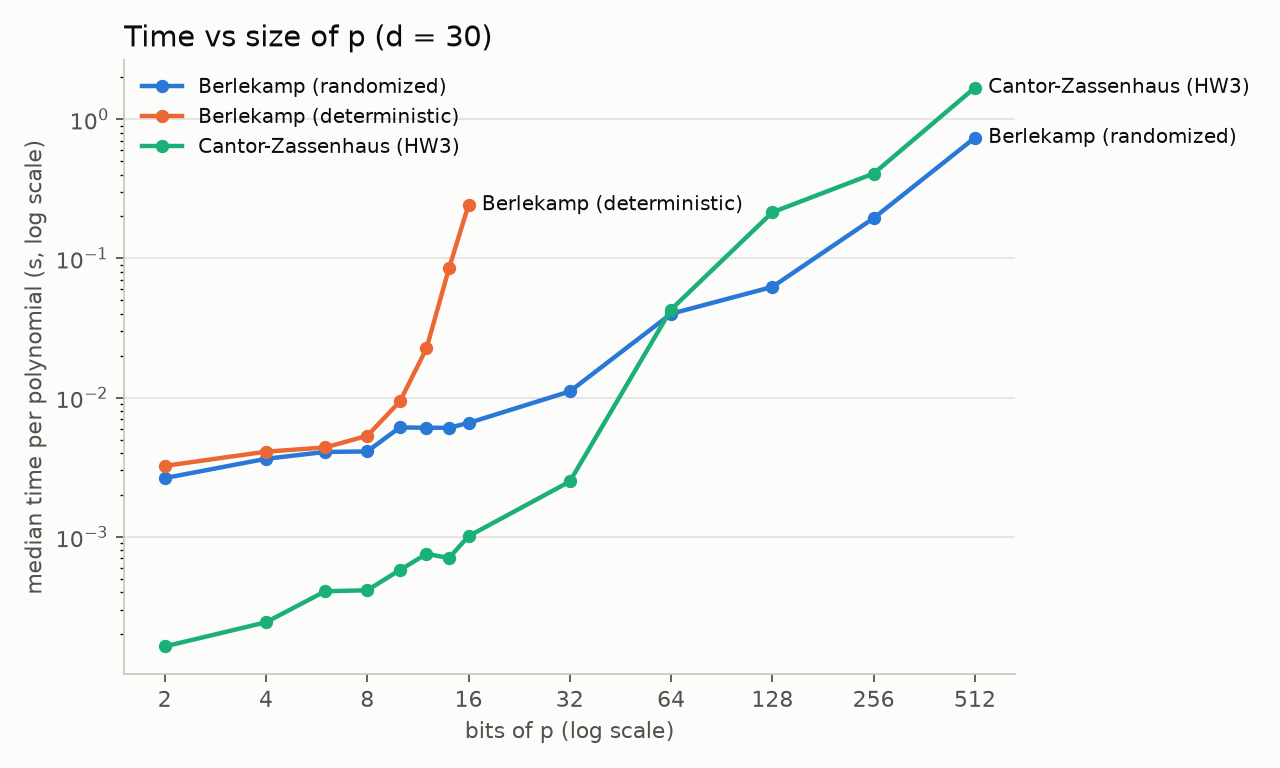
\includegraphics[width=0.78\textwidth]{../bench/results/time_vs_p.png}
\caption{Time versus the number of bits of $p$ ($d = 30$, log scale).}
\end{figure}

\textbf{Observations.}
\begin{itemize}
    \item The deterministic split grows with $p$ itself: from 12 to 16 bits ($p$ grows $16\times$) its time grows about $11\times$. This is the $O(r\,p\,d^2)$ term of Section~4.6 made visible, and it is why the method cannot reach cryptographic sizes.
    \item The randomized split grows only with $\log p$: from 2 to 512 bits its time grows about $280\times$ while $p$ grows by a factor of $2^{510}$.
    \item The two methods are about even at 64 bits ($0.040$ s against $0.043$ s); from 128 bits upward randomized Berlekamp clearly beats our Cantor-Zassenhaus on the same inputs ($0.74$ s against $1.68$ s at 512 bits), as predicted: one exponentiation by $p$ against up to $d/2$ of them. For small $p$ Cantor-Zassenhaus wins, because exponentiations are cheap and Berlekamp's linear algebra dominates.
    \item Sage stores polynomials with FLINT for $p < 2^{63}$ and with NTL above, so part of the jump between 32 and 64 bits comes from the library, not the algorithm.
\end{itemize}

\subsection*{6.4 Time versus degree, and where the time goes}

\begin{table}[H]
\centering
\small
\begin{tabular}{rrrr|rrr}
\toprule
 & \multicolumn{3}{c|}{all methods} & \multicolumn{3}{c}{Berlekamp stages} \\
$d$ & Berlekamp (rand.) & C-Z (HW3) & Sage & build $Q$ & kernel & split \\
\midrule
10  & 0.0007 & 0.0002 & 0.0001 & 0.0002 & 0.0003 & 0.0002 \\
30  & 0.0065 & 0.0009 & 0.0002 & 0.0011 & 0.0049 & 0.0005 \\
50  & 0.0248 & 0.0026 & 0.0006 & 0.0029 & 0.0213 & 0.0008 \\
70  & 0.0633 & 0.0060 & 0.0013 & 0.0056 & 0.0568 & 0.0008 \\
100 & 0.1768 & 0.0105 & 0.0025 & 0.0112 & 0.1627 & 0.0017 \\
\bottomrule
\end{tabular}
\caption{Median time in seconds at $p = 987013$.}
\label{tab:d}
\end{table}

\begin{figure}[H]
\centering
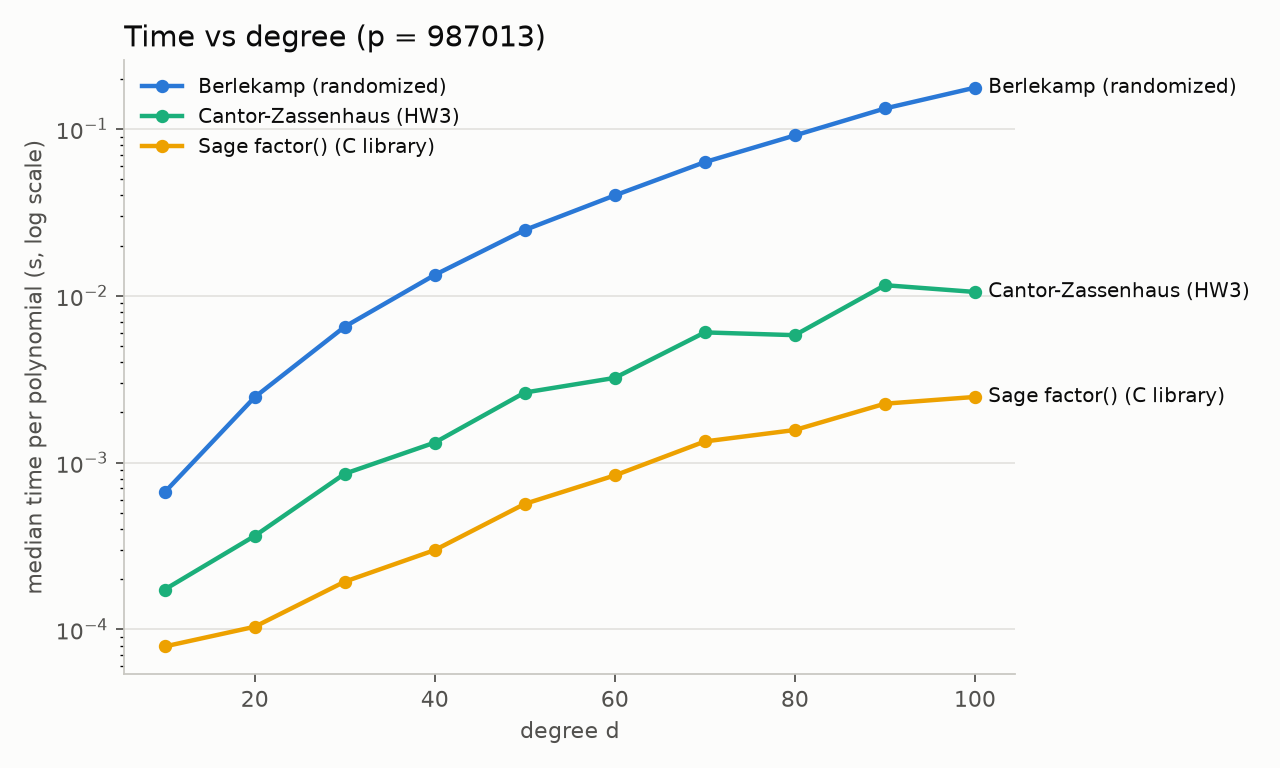
\includegraphics[width=0.49\textwidth]{../bench/results/time_vs_degree.png}
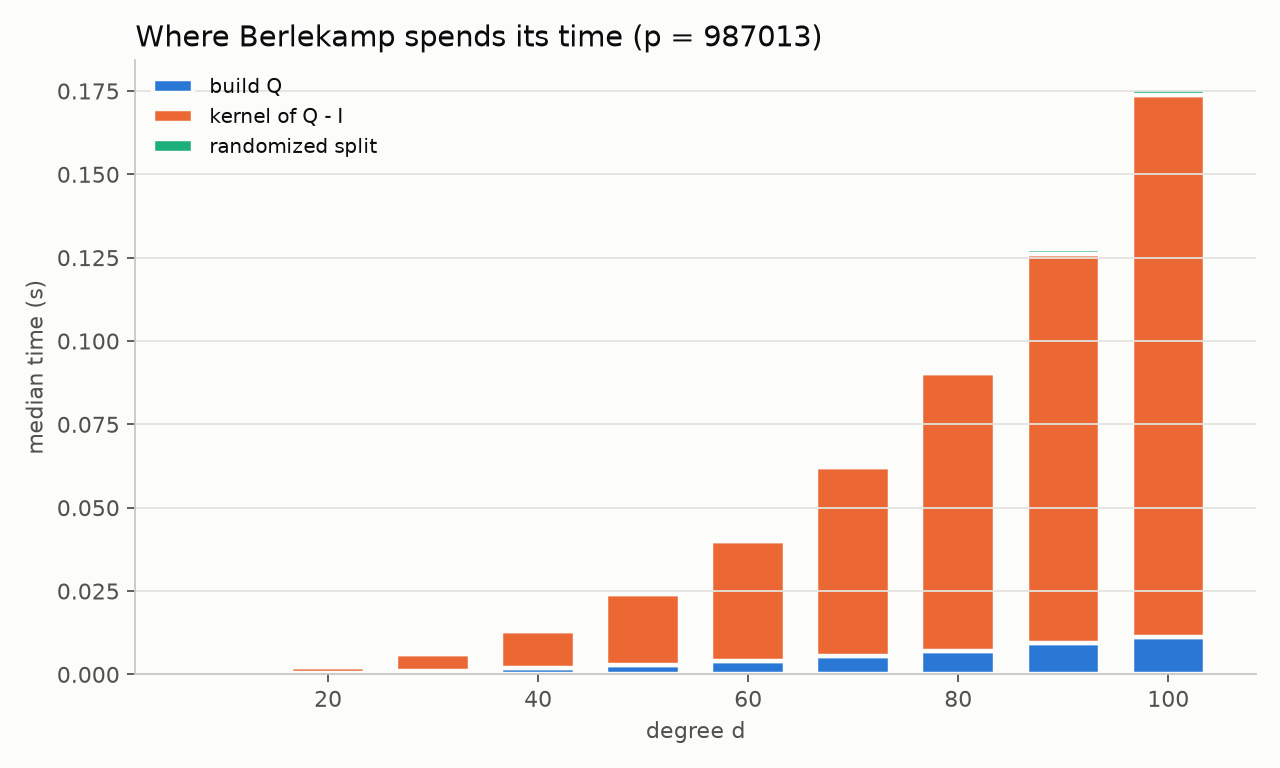
\includegraphics[width=0.49\textwidth]{../bench/results/berlekamp_stages.png}
\caption{Left: time versus degree at $p = 987013$. Right: Berlekamp's time split by stage.}
\end{figure}

At a 20-bit prime, Cantor-Zassenhaus is faster for every degree, and the gap widens with $d$.
The stage breakdown explains why: the kernel of $Q - I$ takes \textbf{over 90\%} of Berlekamp's time
at $d = 100$ and grows like $d^3$, while building $Q$ and splitting are cheap. Our elimination runs
in Python while Cantor-Zassenhaus spends its time in compiled polynomial arithmetic, so the
constant factor is also against Berlekamp here. The fast variants (Section~3) attack exactly this
step.

% -------------------------------------------------------
\section*{7. Discussion and Limitations}
% -------------------------------------------------------

\begin{itemize}
    \item \textbf{What Berlekamp gives that Cantor-Zassenhaus does not.} The number of irreducible factors $r = \dim\ker(Q - I)$ is known after one linear-algebra step, which also gives an irreducibility test. Cantor-Zassenhaus learns the factor degrees only as distinct-degree factorization proceeds.
    \item \textbf{Deterministic is not polynomial time.} The deterministic split is polynomial in $p$, not in $\log p$, so it does not answer the open question of deterministic polynomial-time factoring over $\Zp$; it is practical only for small $p$.
    \item \textbf{Constant factors.} The comparison is fair in arithmetic (same library, same inputs) but not in linear algebra, which is in Python; a compiled elimination would move the crossover in Table~\ref{tab:d} but not the asymptotics.
    \item \textbf{Prime fields only.} Extension fields $\mathbb{F}_{p^k}$ need $Q$ built from the $p^k$-power map; our input check rejects them.
\end{itemize}

% -------------------------------------------------------
\section*{8. Work Split}
% -------------------------------------------------------

\begin{itemize}
    \item \textbf{Member 1 (setup and $Q$):} input and output, square-free decomposition including the $h^p$ case, repeated squaring, the matrix $Q$.
    \item \textbf{Member 2 (kernel and deterministic split):} Gaussian elimination over $\Zp$, Theorem~\ref{thm:dim}, the deterministic split and the driver.
    \item \textbf{Member 3 (large $p$ and evaluation):} the randomized split and its probability analysis, the test suite and the cross-check against Sage, the Cantor-Zassenhaus baseline and the benchmarks.
\end{itemize}

% -------------------------------------------------------
\section*{9. Conclusion}
% -------------------------------------------------------

We implemented Berlekamp's algorithm over $\Zp$ end to end, including square-free decomposition
in characteristic $p$, the matrix $Q$, our own null-space computation, and both the deterministic
and the randomized split. It factors every tested input exactly as Sage does, from $p = 2$ to a
512-bit prime. The experiments confirm the theory: the dimension of $\ker(Q - I)$ counts the
factors, the deterministic split scales with $p$ rather than $\log p$, and randomized Berlekamp
overtakes Cantor-Zassenhaus once $p$ is large compared with $d$, while its $O(d^3)$ linear algebra
makes it slower for high degree.

The code, tests, benchmark results and presentation notebook are in the project repository; the
command \texttt{python -m kersplit --trace < examples/x4plus1\_mod3.txt} reproduces the worked
example of Section~4.7.

\begingroup
\footnotesize
\setlength{\parskip}{0pt}

\begin{thebibliography}{9}
\setlength{\itemsep}{1pt}
\setlength{\parsep}{0pt}

\bibitem{berlekamp67}
E.~R. Berlekamp,
``Factoring Polynomials over Finite Fields,''
\emph{Bell System Technical Journal}, 46(8):1853--1859, 1967.

\bibitem{berlekamp70}
E.~R. Berlekamp,
``Factoring Polynomials over Large Finite Fields,''
\emph{Mathematics of Computation}, 24(111):713--735, 1970.

\bibitem{cantorzassenhaus}
D.~G. Cantor and H.~Zassenhaus,
``A New Algorithm for Factoring Polynomials over Finite Fields,''
\emph{Mathematics of Computation}, 36(154):587--592, 1981.

\bibitem{kaltofenshoup}
E.~Kaltofen and V.~Shoup,
``Subquadratic-Time Factoring of Polynomials over Finite Fields,''
\emph{Mathematics of Computation}, 67(223):1179--1197, 1998.

\bibitem{knuth}
D.~E. Knuth,
\emph{The Art of Computer Programming, Vol.~2: Seminumerical Algorithms}, 3rd ed., Section 4.6.2,
Addison-Wesley, 1997.

\bibitem{shoup}
V.~Shoup,
\emph{A Computational Introduction to Number Theory and Algebra}, 2nd ed., Chapter 20,
Cambridge University Press, 2009.

\bibitem{mca}
J.~von zur Gathen and J.~Gerhard,
\emph{Modern Computer Algebra}, 3rd ed., Chapter 14, Cambridge University Press, 2013.

\bibitem{notes}
N.~R. Aravind,
CS5610 course notes, Chapters 6--7 (finite fields, Cantor-Zassenhaus, CRT for polynomials),
IIT Hyderabad, 2026.

\end{thebibliography}
\endgroup

\end{document}
